\documentclass[11pt,a4paper]{article}

\usepackage{../riddle}
\usepackage[maxalphanames=99, maxnames=99, backend=bibtex, style=alphabetic, sorting=ynt]{biblatex}
\addbibresource{stage3A.bib}
\DeclareSymbolFont{yhlargesymbols}{OMX}{yhex}{m}{n} 
\DeclareMathAccent{\yhwidehat}{\mathord}{yhlargesymbols}{"62}
\renewcommand{\headrulewidth}{1pt} 
\renewcommand{\footrulewidth}{1pt}	
\fancyhead[C]{}
\fancyhead[L]{}
\fancyhead[R]{}
\fancyfoot[C]{\thepage} 
\fancyfoot[L]{Sacha Ben-Arous}
\fancyfoot[R]{E.N.S Paris-Saclay}
\usepackage{tikz-cd}
\usepackage{subcaption}
\setlength{\parindent}{0pt}

% Majda-Bertozzi avec fiches -> Eggers-Fontelos -> Tao chap1 et annexe -> papier et articles connexes 

% https://www.youtube.com/watch?v=mw_hhOqKDx4 (T.B. intro papier 2D)
% https://vimeo.com/539376697/bbc4763e80 (T.B. intro papier 3D)
% https://www.youtube.com/watch?app=desktop&v=JRBwdVFmcE4 (T.B. exemple conf avec op linéarisé) (en chercher d'autres)


%TODO SE REFERER AU DOCUMENT DE F PI !!!!!!!!!

%TODO : Classification AMS

%TODO : tout check puis partie anglais


\begin{document}

\begin{titlepage}
\centering
\vspace*{0.5cm}
{\large École Normale Supérieure Paris-Saclay \par}
{\large New York University, Courant Institute \par}
\vspace{1cm}
{\large Research internship conducted as part of the Master 1 Hadamard \par}
{\large Supervised by Tristan Buckmaster\par}

\vspace{3cm}
{\Huge \textbf{Self-similar singularity formation in fluids}\par}
\vspace{1cm}

{\Large {Sacha Ben-Arous}\par}
    \vfill 
     \begin{tabular}{p{0.45\linewidth} p{0.45\linewidth}}
        \raisebox{-1.6cm}{
\includegraphics[width=7cm]{logo_accueil.png}} & 
        \hfill 
\includegraphics[scale=0.25]{logo_origine.jpg}
    \end{tabular}

\end{titlepage}
{\centering
\section*{Compte-rendu de stage}
}
\hspace*{2em} D'avril à août 2025, j'ai effectué mon stage de Master 1 à l'Université de New York, sous la direction de Tristan Buckmaster. Ce stage avait pour objectif à la fois de m'initier à un domaine de recherche (très) actif, et de découvrir le fonctionnement du monde de la recherche. Le compte-rendu qui suit décrit mon expérience globale au cours de ce stage. \\

\hspace*{2em} Tout d'abord, ce qui m'a attiré vers ce stage est la possibilité de d'étudier un problème central des mathématiques : le caractère bien-posé de certaines équations de la mécanique des fluides, sous la direction d'un chercheur ayant apporté des contributions significatives à ce domaine : Tristan Buckmaster a participé à la résolution de la conjecture d'Onsager, avec P. Isett et V. Vicol. De plus, le Courant Institute où j'ai effectué mon stage a une grande tradition de l'étude théorique et numérique de la mécanique des fluides, grâce à d'illustres mathématiciens  tels que P. Lax, L. Nirenberg, A. Majda, C. Morawetz, et plus récemment avec T. Buckmaster, V. Vicol, J. Shatah. \\

\hspace*{2em} Par ailleurs, j'ai dès le début de mon stage été marqué par la pluridisciplinarité présente dans ce laboratoire, grâce au large spectre de disciplines représentées. Un nombre colossal d'exposés avaient lieu durant le premier mois de stage (au moins un par jour), dont les sujets variaient de l'étude numérique appliquée de la dynamique des océans jusqu'à l'utilisation de matrices aléatoires pour étudier la fonction zêta de Riemann, en passant par de la théorie de la mesure géométrique, avec la fameuse résolution de la conjecture de Kakeya par Hong Wang en Mars dernier. \\
\hspace*{2em} Un autre fait marquant a été d'assister à la conférence célébrant la retraite de S.R.S. Varadhan, monument des probabilités modernes, ayant passé 60 ans (!!!) au Courant Institute, en ayant été deux fois son directeur. Ce dernier est à l'origine de l'autre tradition majeure de Courant : l'étude et le développement de la théorie des probabilités modernes, en particulier des phénomènes de grandes déviations, ainsi que de l'étude des processus de diffusion. Cette conférence a été l'occasion pour moi de découvrir des facettes souvent négligées dans les descriptions des grandes carrières scientifiques : Varadhan a bien sûr été extrêmement prolifique sur le plan des découvertes mathématiques, mais il s'est aussi et surtout massivement investi dans la construction d'une culture de la recherche en probabilité qui porte encore ses fruits aujourd'hui, par exemple avec l'étude des matrices aléatoires citée ci-dessus, mais aussi avec l'intelligence artificielle, qui est aujourd'hui sans conteste le domaine le plus actif de la recherche mathématique, et dans lequel le Courant Institute est un lieu d'avant garde. \\
\hspace*{2em} Finalement, j'ai aussi eu la chance de participer  à la fin de mon stage à une summer school organisée par la National Science Foundation, portant précisement sur le thème de mon stage, qui se déroulait au département de mathématiques de Princeton. Cela m'a permis d'avoir d'être exposé à des travaux actuels, d'avoir de très nombreuses discussions avec les différents participants, qu'ils soient professeurs ou élèves, et d'observer comment se coordonne un groupe de recherche en établissant une stratégie à long terme pour résoudre un problème important. \\

\hspace*{2em} Concernant le contenu de mon stage, j'ai été initié à une stratégie très générale employée par Tristan Buckmaster et ses collaborateurs permettant de prouver l'existence de solutions singulières aux équations de la mécanique des fluides, telles que l'équation d'Euler ou l'équation de Navier-Stokes (incompressibles). Ce problème est bien sur très célèbre, car il est mis à prix par le Clay Institute pour un million de dollars, David Hilbert l'ayant décrit comme l'un des problèmes devant guider les recherches des mathématiciens au cours de notre millénaire. Ce problème peut à première vue sembler dénué d'interêt aujourd'hui, tant les modélisations utilisées dans des domaines appliquées tels que la météorologie ou l'étude de la dynamique des océans sont infiniments plus compliquées. Cependant, ce qui motive une telle question n'est pas d'évaluer la pertinence des équations d'Euler ou de Navier-Stokes pour décrire la réalité, mais est plutôt de permettre, via l'abstraction induite par le cadre mathématique, de mettre en évidence les potentielles incohérences et défauts de nos modélisations intuitives des fluides conduisant à des absurdités physiques, et donc de repenser à un niveau fondamental notre conception et appréhension des fluides. Le premier résultat majeur sur ce sujet a été publié par Jean Leray en 1934 \cite{leray1934} dans lequel est établi l'existence globale de solutions faibles, "turbulentes", aux équations de Navier-Stokes, aujourd'hui appelées solutions de Leray-Hopf. Ce sujet a été largement étudié depuis, et une avancée importante récente est l'existence de données initiales lisses qui conduisent à une singularité pour l'équation d'Euler à frontière cylindrique, publiée par Chen et Hou en 2023 dans une série d'articles \cite{chen_hou1},\cite{chen_hou2}, et qui utilise une stratégie semblable à celle décrite dans ce rapport. \\
\hspace*{2em} Il faut aussi noter le récent progrès dans la résolution du 6ème problème de Hilbert, qui concerne la dérivation probabiliste des équations de la physique (en particulier de la mécanique des fluides), obtenu par Deng, Hani, Ma \cite{deng_hani_ma_2025_hilbert6}. Ce résultat s'inscrit dans une série de travaux menés par Bodineau, Gallagher, Golse, Saint-Raymond, et offre une approche potentiellement différente de la vision analytique classique, car elle s'appuie sur des outils probabilistes, et est motivée physiquement par la description atomique, moléculaire, des fluides. Cette vision probabiliste des fluides comme étant la limite d'un ensemble de particules en interaction ne sera cependant pas abordée ici. \\

\hspace*{2em} D'un point de vue pratique, j'ai d'abord commencé par apprendre les résultats classiques de la mécanique des fluides et de l'auto-similarité dans des livres tels que \cite{majda2001vorticity}, \cite{eggers2015singularities}, \cite{tao2006dispersive}, j'ai ensuite lu les articles \cite{buckmaster2019formation},\cite{buckmaster2022imploding} afin de découvrir les différentes techniques utilisées pour résoudre le type de problème auquel j'étais confronté. J'ai ensuite expérimenté avec les approximations numériques et l'utilisation des bibliothèques Python de calcul formel et de calculs rigoureux, puis j'ai appliqué la méthode générale précédemment mentionnée dans le cas de l'équation de Burgers. \\

\hspace*{2em} Finalement, je souhaite remercier les doctorants avec lesquels j'ai été amené à travailler : Grayson Davis, Chen Li, et Kaiwen Zhang. Ils m'ont accompagné tout au long du stage, et les résultats présentés dans ce document sont issus d'un travail de groupe que nous avons mené ensemble.

\newpage
{\centering
\section*{Internship summary}
}
\hspace*{2em} From April to August 2025, I carried out my Master 1 internship at New York University, under the supervision of Tristan Buckmaster. The aim of this internship was both to introduce me to a (very) active field of research, and to discover how the world of research operates. The following report describes my overall experience during this internship. \\

\hspace*{2em} First of all, what attracted me to this internship was the opportunity to study a central problem in mathematics: the well-posedness of certain equations in fluid mechanics, under the guidance of a researcher who has made significant contributions to this field: Tristan Buckmaster took part in the resolution of Onsager’s conjecture, along with P. Isett and V. Vicol. Moreover, the Courant Institute, where I did my internship, has a great tradition of theoretical and numerical study of fluid mechanics, thanks to illustrious mathematicians such as P. Lax, L. Nirenberg, A. Majda, C. Morawetz, and more recently T. Buckmaster, V. Vicol, J. Shatah. \\

\hspace*{2em} Furthermore, I was struck right from the beginning of my internship by the interdisciplinarity present in this laboratory, thanks to the wide spectrum of represented disciplines. An enormous number of talks took place during the first month (at least one per day), with subjects ranging from applied numerical study of ocean dynamics to the use of random matrices to study the Riemann zeta function, including geometric measure theory, with the famous resolution of the Kakeya conjecture by Hong Wang last March. \\
\hspace*{2em} Another striking event was attending the conference celebrating the retirement of S.R.S. Varadhan, a monument of modern probability, who spent 60 years (!!!) at the Courant Institute, serving twice as its director. He is at the origin of Courant’s other major tradition: the study and development of modern probability theory, in particular large deviations phenomena, as well as the study of diffusion processes. This conference was for me the occasion to discover aspects often neglected in the descriptions of great scientific careers: Varadhan was of course extremely prolific in terms of mathematical discoveries, but he also, and above all, invested massively in building a culture of research in probability that still bears fruit today, for instance with the study of random matrices mentioned above, but also with artificial intelligence, which is nowadays without doubt the most active field in mathematical research, and in which the Courant Institute is a leading place. \\
\hspace*{2em} Finally, I also had the chance, at the end of my internship, to participate in a summer school organized by the National Science Foundation, focusing precisely on the subject of my internship, which took place at the Department of Mathematics at Princeton. This allowed me to be exposed to current work, to have many discussions with different participants, whether professors or students, and to observe how a research group coordinates by establishing a long-term strategy to solve an important problem. \\

\hspace*{2em} Regarding the content of my internship, I was introduced to a very general strategy employed by Tristan Buckmaster and his collaborators, allowing one to prove the existence of singular solutions to the equations of fluid mechanics, such as the Euler equation or the (incompressible) Navier–Stokes equation. This problem is of course very famous, since it has been awarded a one-million-dollar prize by the Clay Institute, David Hilbert having described it as one of the problems meant to guide mathematicians’ research during our millennium. At first glance, this problem may seem devoid of interest today, given that the models used in applied fields such as meteorology or the study of ocean dynamics are infinitely more complicated. However, what motivates such a question is not to assess the relevance of the Euler or Navier–Stokes equations in describing reality, but rather to use the abstraction induced by the mathematical framework to highlight the potential inconsistencies and flaws of our intuitive models of fluids that lead to physical absurdities, and thus to rethink at a fundamental level our conception and understanding of fluids. The first major result on this subject was published by Jean Leray in 1934 \cite{leray1934}, establishing the global existence of weak, “turbulent” solutions to the Navier–Stokes equations, today called Leray–Hopf solutions. This subject has been widely studied since then, and an important recent advance is the existence of smooth initial data leading to a singularity for the Euler equation with cylindrical boundary, published by Chen and Hou in 2023 in a series of articles \cite{chen_hou1}, \cite{chen_hou2}, which uses a strategy similar to the one described in this report. \\
\hspace*{2em} It is also worth noting the recent progress in the resolution of Hilbert’s 6th problem, which concerns the probabilistic derivation of the equations of physics (in particular fluid mechanics), obtained by Deng, Hani, Ma \cite{deng_hani_ma_2025_hilbert6}. This result belongs to a series of works led by Bodineau, Gallagher, Golse, Saint-Raymond, and offers a potentially different approach from the classical analytical view, since it relies on probabilistic tools and is physically motivated by the atomic, molecular description of fluids. However, this probabilistic vision of fluids as the limit of a set of interacting particles will not be discussed here. \\

\hspace*{2em} From a practical point of view, I first started by learning the classical results of fluid mechanics and self-similarity in books such as \cite{majda2001vorticity}, \cite{eggers2015singularities}, \cite{tao2006dispersive}. I then read the articles \cite{buckmaster2019formation}, \cite{buckmaster2022imploding} in order to discover the different techniques used to solve the type of problem I was faced with. I then experimented with numerical approximations and the use of Python libraries for symbolic and rigorous computation, and then I applied the general method previously mentioned in the case of the Burgers equation. \\

\hspace*{2em} Finally, I would like to thank the PhD students with whom I had the opportunity to work: Grayson Davis, Chen Li, and Kaiwen Zhang. They accompanied me throughout the internship, and the results presented in this document stem from a group effort we carried out together.
\newpage
\tableofcontents
\newpage
{\centering\section*{Abstract}}
\hspace*{2em} In this document, I will present a general method to prove the existence of a large set of initial data that leads to the blowup of some PDE, by exhibiting a "universal" blowup profile. This type of result is remarkable since it suggests that the structure of the blowup has some physical meaning, as opposed to some famous blowup results where the initial data is crafted using non-measurable sets, or functions that are not even in the category of distributions.
In the first section, I will present basic results about the Burgers equation, which will be the example studied throughout the report. In the second part, I will present the core of the strategy and apply it to Burgers' equation. This constitutes my personal work during the internship, with the collaboration of the aforementioned phd students. In the conclusion, I will briefly discuss the strategy in the setting of a harder equation, and what are the new tools used in such cases. \\


\section{Introduction to self-similar analysis}
\hspace*{2em} In this section, I will present the concepts of shock formation and self-similar blow-up for a nonlinear partial differential equation, illustrated by the fundamental example of Burgers' equation. The references for this section are  \cite{majda2001vorticity} and \cite{eggers2015singularities}.

\subsection{Characteristics for Burgers' equation}
\hspace*{2em} We will say that there is a blowup or a singularity when a quantity of the equation goes to infinity. Recall Burgers' equation:
\label{burgers}
\begin{equation}
\begin{cases} \partial_t u + u\partial_x u = 0 \\ u(x,0)=u_0 \end{cases}
\end{equation}

\noindent This is the simplest case of a nonlinear transport equation. Indeed, if one changes the term $u\partial_x u$ by $v\partial_x u$ where $v$ is some positive constant, then the solution to this equation is just the initial profile $u_0$ shifted at speed $v$ in time: $u(x,t) = u_0(x - v t)$.
In the general nonlinear case, one can solve this equation by the method of characteristics. For some $x_0\in \R$, define the characteristics curve:  \[\eta_{x_0}(t) :=x_0+ u_0(x_0)t.\]

\noindent Apply the chain rule along this trajectory to the composition $t\mapsto u(\eta_{x_0}(t),t)$:
\[
\frac{\mathrm{d}}{\mathrm{d}t} \Big(u\big(\eta_{x_0}(t),t\big)\Big)
=\partial_t u\big(\eta_{x_0}(t),t\big)+\eta_{x_0}'(t)\,\partial_x u\big(\eta_{x_0}(t),t\big).
\]
Using the PDE \eqref{burgers}, we obtain
\[
\frac{\mathrm{d}}{\mathrm{d}t}u\big(\eta_{x_0}(t),t\big)
=\partial_t u + u\,\partial_x u = 0.
\]
Therefore $u$ is constant along each characteristic, and
\begin{equation}\label{const_along}
u\big(\eta_{x_0}(t),t\big)=u_0(x_0)\quad\text{for all }t\ge0.
\end{equation}

\noindent When characteristics intersects, the function $u$ is multi-valued, implying that there is a singularity. This first happens when the map
\[x_0\mapsto x=x_0+u_0(x_0)t\]
is no longer injective, since it is required in order to recover $x_0$ from $(x,t)$ and thus define $u(x,t)$ by \eqref{const_along}. Its derivative with respect to $x_0$ is
\[
\frac{\partial x}{\partial x_0}=1+t\,u_0'(x_0).
\]
Consequently the classical solution exists while
\[1+t\,u_0'(x_0)>0\quad\text{for all }x_0.
\]
If $u_0'$ takes negative values, then characteristics intersects and a shock forms. In that case, the earliest time of breakdown is
\begin{equation}\label{break_time}
t_* = \min_{\{x_0:\;u_0'(x_0)<0\}}\left(-\frac{1}{u_0'(x_0)}\right)
= -\frac{1}{\inf_{x_0}u_0'(x_0)}\qquad\text{(provided }\inf_{x_0}u_0'(x_0)<0\;).
\end{equation}

\noindent Denoting $x_m$ the point where the minimum is reached,  \eqref{const_along} tells us that the singularity will form at the point $x_* := x_m - \frac{u_0(x_m)}{u_0'(x_m)}$. \\
After $t_*$ one must pass to entropy solutions and use methods such as the Rankine--Hugoniot condition to determine the shock speed and the continuation of the solution, but we will not discuss this.

\begin{figure}[ht]
  \centering
  \begin{subfigure}[b]{0.32\textwidth}
    \raisebox{0.2cm}{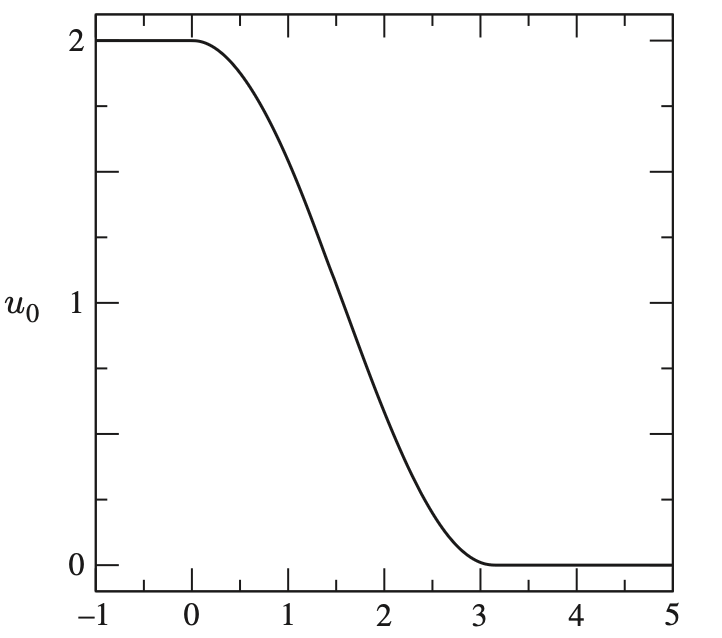
\includegraphics[width=\linewidth]{char1.png}}
    \caption{Initial profile}
  \end{subfigure}\hfill
  \begin{subfigure}[b]{0.32\textwidth}
    \raisebox{0cm}{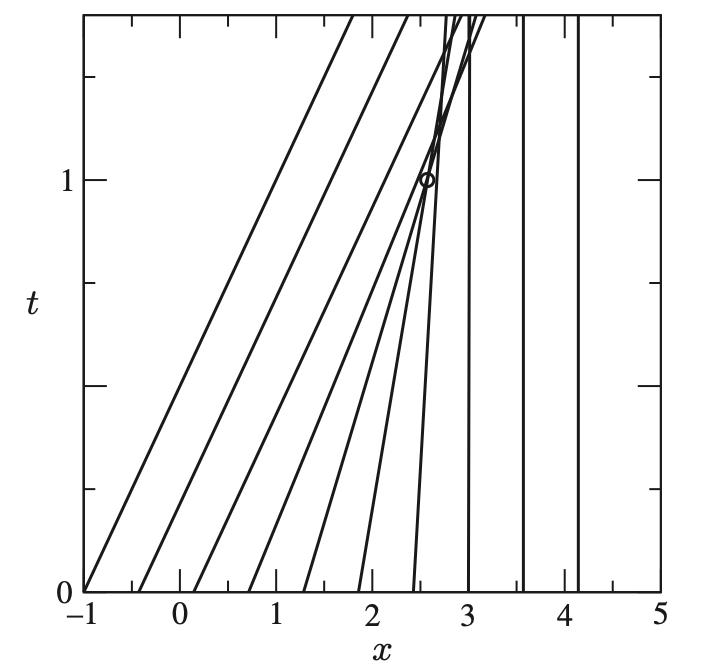
\includegraphics[width=\linewidth]{char2.png}}
    \caption{Characteristic lines}
  \end{subfigure}\hfill
  \begin{subfigure}[b]{0.32\textwidth}
    \raisebox{0cm}{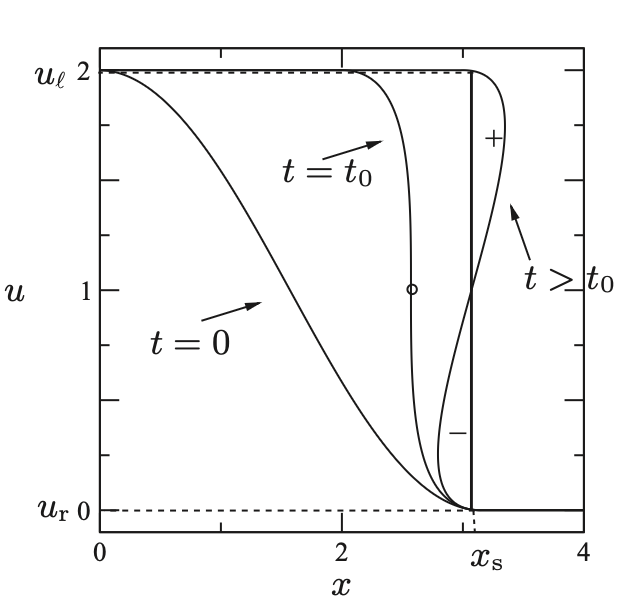
\includegraphics[width=\linewidth]{char3.png}}
    \caption{Profiles near the blowup}
  \end{subfigure}
  \caption{Blowup of a smooth profile illustrated by characteristics \cite{eggers2015singularities}}
\end{figure}


\subsection{The self-similar equation}
The notion of self-similarity goes back to Leray's seminal paper \cite{leray1934}. Its main purpose is to transform a singular problem into a smooth one, as we explain below. \\

\noindent Let $u$ be a solution of \eqref{burgers}, $\alpha$ and $\beta$ be real numbers, and define $U$ the self-similar ansatz
\begin{equation}
    u(x', t') = (t')^\alpha U(\xi), \text{ where }\xi = \frac{x'}{(t')^\beta}, t' = t_* - t, x'=x-x_*
\end{equation}

Here, $t_*, x_*$ are viewed as the time and location of singularity formation. The purpose of this self-similar change of coordinates is to regularize a singular problem. This is not contradictory, since the change of variables itself is singular. \\

We impose for now two conditions on $U$ for admissible solutions:
\begin{itemize}
    \item $u(x', t')$ must grow slowly without blowup for any $x'\ne 0$ (away from the blowup point)
    \item $U$ must be "regular" for all $\xi$
\end{itemize}

More precisely for the first condition, we ask that
\begin{equation}
    \lim_{t'\to 0} u(x', t') = \lim_{t'\to 0}(t')^\alpha U\left(\frac{x'}{(t')^\beta}\right) \text{ is finite } \forall x'\ne 0
\end{equation}

Writing $(t')^\alpha$ in terms of $\xi$ we learn that 
\begin{align*}
    \lim_{t'\to 0} u(x', t') &= \lim_{t'\to 0} \left[\frac{x'}{(t')^\beta}\right]^{-\frac{\alpha}{\beta}}\cdot (x')^{\frac{\alpha}{\beta}}\cdot U\left(\frac{x'}{(t')^\beta}\right) \\
    &\simeq \lim_{\xi\to\pm\infty} \xi^{-\frac{\alpha}{\beta}} U(\xi) <\infty
\end{align*}

And hence 
\begin{equation}\label{eq:matching-cond}
    \lvert U(\xi)\rvert \le C \lvert \xi\rvert ^{\frac{\alpha}{\beta}} \text{ as } \xi\to\pm\infty
\end{equation}

\subsection{Similarity equation and solutions}

To substitute this ansatz into \eqref{burgers}, we use chain rule and the fact that $\frac{x'}{(t')^{\beta +1}} = \frac{\xi}{t'}$ to compute and obtain
\begin{align*}
    \frac{\partial u}{\partial t} &= -\alpha(t')^{\alpha-1}U(\xi) + (t')^\alpha U'(\xi) \frac{x'\beta}{(t')^{\beta +1}} =-\alpha (t')^{\alpha-1}U(\xi) + (t')^\alpha \beta\frac{\xi}{t'}U'(\xi) \\
    &=(t')^{\alpha-1}(-\alpha U(\xi) + \beta \xi U'(\xi))
\end{align*}

\begin{align*}
    \frac{\partial u}{\partial x}=(t')^{\alpha-\beta}U'(\xi)
\end{align*}

Thus $$uu_x = (t')^{2\alpha-\beta}U(\xi)U'(\xi)$$ For $u_t$ and $uu_x$ to have matching power on $t'$, we determine that $\beta = \alpha+1$. 

Then for times before the singularity, we arrive at the \textbf{similarity equation}:
\begin{equation}\label{eq:sim-eq}
    -\alpha U(\xi) + (\alpha+1)\xi U'(\xi) + U(\xi) U'(\xi) = 0
\end{equation}

To solve it, first rearrange to 
$$U'(\xi) = \frac{\alpha U(\xi)}{(\alpha+1)\xi + U(\xi)}$$ 
Then seeing the difficulty in separating variables, the trick is to view $\xi$ as the dependent variable and write 
$$\xi'(U) = \frac{1}{\alpha} + \frac{\alpha+1}{\alpha}\frac{1}{U}\xi(U)$$ 
resulting in the linear ODE 
$$\xi'(U) - (1+\frac{1}{\alpha})\frac{1}{U}\xi(U) = \frac{1}{\alpha}$$ 
The homogeneous part has general solution $\xi^h(U) = CU^{1+\frac{1}{\alpha}}$. Then, observing that $\xi^*(U) = -U$ is a special solution to the inhomogeneous equation, we conclude the general implicit solution to \ref{eq:sim-eq} is 

\begin{equation}\label{eq:sim-sol-im}
    \xi = -U + CU^{1+\frac{1}{\alpha}}
\end{equation}

Note that we can rule out the case of $\alpha = 0$ because the corresponding solution is $\xi = -U$ does not satisfy the decay condition \ref{eq:matching-cond}.

Next we impose the regularity condition, for $U(\xi)$ to be smooth, $1+\frac{1}{\alpha}$ must be a positive integer (fractional powers eventually lead to negative powers in derivatives); for the expression \ref{eq:sim-sol-im} to be invertible, $1+\frac{1}{\alpha}$ must be odd. Hence we arrive at an array of admissible values for $\alpha$:

\begin{equation}
    \alpha_i = \frac{1}{2i+2}, i = 0,1,2,...
\end{equation}

Note that for each finite $\alpha$ we would have $U^{1+\frac{1}{\alpha}}\sim \xi$, so $U\sim \xi^{\frac{\alpha}{\alpha+1}}$, satisfying the decay condition.

For the case $i = 0, \alpha = \frac{1}{2}$, $U$ can be explicitly computed as:
\begin{equation}\label{eq:exact-profile}
    U(x) = \left(-\frac{x}{2} + \sqrt{\frac{1}{27}+\frac{x^2}{4}}\right)^{\frac{1}{3}} - \left(\frac{x}{2} + \sqrt{\frac{1}{27}+\frac{x^2}{4}}\right)^{\frac{1}{3}} 
\end{equation}
However, in more complicated problems we should not expect to see such exact results.

\subsection{Stability and the linearized operator}
We want to state the singularity formation problem in terms of some sort of convergence of solution to the self-similar profile. To achieve this, it helps to transform finite-time singularity formation to a problem of long time stability, we introduce a new time coordinate: $\tau := -\log t'$. Then as $t'\to 0$, $\tau \to \infty$.

We write, with the change of variables $\xi = \frac{x'}{(t')^{\alpha+1}}, \tau = -\log t'$,
\begin{equation}\label{eq:ansatz-sim-coor}
    u(x', t') = (t')^\alpha U(\xi, \tau) = e^{-\tau} U(\xi, \tau)
\end{equation}

From the original equation \eqref{burgers}, compute using chain rule and the relation $\xi = \frac{x'}{(t')^{\alpha+1}}$
\begin{align*}
    \frac{\partial u}{\partial t} &= -\alpha (t')^{\alpha-1} U(\xi, \tau) + (t')^\alpha \frac{\partial U}{\partial\tau}\cdot\frac{\partial\tau}{\partial t} + (t')^\alpha \frac{\partial U}{\partial\xi}\cdot\frac{\partial\xi}{\partial t}\\
    &= -\alpha (t')^{\alpha-1} U(\xi, \tau) + (t')^\alpha U_\tau(\xi, \tau)\cdot\left(\frac{-1}{-t'}\right) + (t')^\alpha U_\xi(\xi, \tau)\cdot\left(\frac{x'(\alpha+1)}{(t')^{\alpha+2}}\right) \\
    &= -\alpha (t')^{\alpha-1} U(\xi, \tau) + (t')^{\alpha-1} U_\tau(\xi, \tau) + (t')^{\alpha-1} \frac{\xi}{t'}(\alpha+1)U_\xi(\xi, \tau)
\end{align*}

and
\begin{align*}
    \frac{\partial u}{\partial x} = (t')^\alpha U_\xi(\xi, \tau)\frac{1}{(t')^{\alpha + 1}}
\end{align*}

to obtain the \textbf{dynamical system equation} for $U(\xi, \tau)$:
\begin{equation}\label{eq:dyn-sys}
    U_\tau - \alpha U + (\alpha+1)\xi U_\xi + UU_\xi = 0
\end{equation}

Notice that any similarity profile $\Bar{U}$ satisfying the similarity equation \ref{eq:sim-eq} automatically has $-\alpha U + (\alpha+1)\xi U_\xi + UU_\xi = 0$ and is hence a fixed point in the dynamical system \ref{eq:dyn-sys}. To perform linear stability analysis around such fixed points, we consider functions of form 
\begin{equation*}
    U(\tau, \xi) = \overline{U}(\xi) + \epsilon P(\tau, \xi)
\end{equation*}

Plug in equation \ref{eq:dyn-sys} to find:
\begin{equation*}
    \epsilon P_\tau = \epsilon \left(\alpha P  -(\alpha + 1)\xi P'(\xi) - \overline{U}(\xi)P'(\xi) - \overline{U}'(\xi) P(\xi)\right) + O(\epsilon^2)
\end{equation*}

Hence the linearized operator that determines the stability of the similarity profile $\overline{U}$ is 
\begin{equation}\label{eq:linearized-op}
    LP(\xi):=\alpha P(\xi) -(\alpha + 1)\xi P'(\xi) - \overline{U}(\xi)P'(\xi) - \overline{U}'(\xi) P(\xi)
\end{equation}

We can also make the situation more explicit by studying a more specific form of perturbation:
$$U(\xi, \tau) = \Bar{U}(\xi) + \delta e^{\nu \tau}P(\xi)$$
and study the sign of $\nu$. 

Substituting this form into equation \ref{eq:dyn-sys}, and recalling that $-\alpha \Bar{U} + + (\alpha+1)\xi \Bar{U}_\xi + \Bar{U}\Bar{U}_\xi = 0$, we arrive at
$$\delta \nu e^{\nu \tau}P(\xi) - \alpha \delta e^{\nu \tau}P(\xi) + (\alpha+1) \xi \delta e^{\nu \tau}P'(\xi) + \Bar{U}(\xi)\cdot \delta e^{\nu \tau}P'(\xi) + \delta e^{\nu \tau}P(\xi)\cdot \Bar{U}'(\xi)=0$$

and after cleaning up we arrive at an eigenproblem for the linearized operator:
\begin{equation*}
    LP(\xi) =\alpha P(\xi) -(\alpha + 1)\xi P'(\xi) - \Bar{U}(\xi)P'(\xi) - \Bar{U}'(\xi) P(\xi) = \nu P(\xi)
\end{equation*}

We can also make the situation more explicit by studying a more specific form of perturbation:
$$U(\xi, \tau) = \Bar{U}(\xi) + \delta e^{\nu \tau}P(\xi)$$
and study the sign of $\nu$. 

Substituting this form into equation \ref{eq:dyn-sys}, and recalling that $-\alpha \Bar{U} + + (\alpha+1)\xi \Bar{U}_\xi + \Bar{U}\Bar{U}_\xi = 0$, we arrive at
$$\delta \nu e^{\nu \tau}P(\xi) - \alpha \delta e^{\nu \tau}P(\xi) + (\alpha+1) \xi \delta e^{\nu \tau}P'(\xi) + \Bar{U}(\xi)\cdot \delta e^{\nu \tau}P'(\xi) + \delta e^{\nu \tau}P(\xi)\cdot \Bar{U}'(\xi)=0$$

and after cleaning up we arrive at an eigenproblem for the linearized operator:
\begin{equation*}
    LP(\xi) =\alpha P(\xi) -(\alpha + 1)\xi P'(\xi) - \Bar{U}(\xi)P'(\xi) - \Bar{U}'(\xi) P(\xi) = \nu P(\xi)
\end{equation*}

We will focus on studying this linearized operator in later sections. We will focus on the case $i = 0, \alpha = \frac{1}{2}$.

\subsection{Family of Solutions and Removal of Symmetries}
Given one solution $u$ to the original equation \eqref{burgers}, one can actually generate a family of solutions. We call such properties "symmetries" of the Burgers equation. 

Suppose $u(x, t)$ is a solution to Burgers' equation \eqref{burgers}. Then so are these:
\begin{itemize}
    \item $v(x,t) := u(x-ct, t)+c$: indeed,
    \begin{align*}
        (v_t + vv_x)(x,t) &= -cu_x(x-ct,t) + u_t(x-ct,t) + (u(x-ct,t)+c)u_x(x-ct,t) \\
        &= (u_t+uu_x)(x-ct,t) = 0
    \end{align*}
    \item $w(x,t) := \lambda u(x,\lambda t)$: indeed,
    \begin{align*}
        (w_t+ww_x)(x,t) = \lambda^2 u_t(x,\lambda t) + \lambda u(x,\lambda t)\cdot \lambda u_x(x,\lambda t) = \lambda^2 (u_t+uu_x)(x,\lambda t) = 0
    \end{align*}
    \item $p(x,t) := \frac{1}{\eta} u(\eta x,t)$: indeed,
    \begin{align*}
        (p_t  + pp_x)(x,t) = \frac{1}{\eta} u_t(\eta x,t) + \frac{1}{\eta} u(\eta x, t)\cdot u_x(\eta x, t) = 0
    \end{align*}
    \item $q(x,t) := u(x-x_0,t)$, this is easy to see.
\end{itemize}

Since we are constructing one solution that blows up, we can make additional restrictions to our initial data to help later analysis. 
\begin{itemize}
    \item $v(x,0) = u(x,0) + c$ - a shift by a constant in the value of initial data
    \item $w(x,0) = \lambda u(x,0)$ - multiplication of initial data by a constant. $\lambda$ can be determined by fixing $u_x(x,0)$
    \item $p(x,0) = \frac{1}{\eta} u(\eta x,0)$ - a spatial scaling of initial data. $\eta$ can be determined by fixing $u_{xx}(x,0)$; the first derivative is not enough.
    \item $q(x,0) = u(x-x_0,0)$ - a translation of initial data. $x_0$ can be fixed with no additional effort.
\end{itemize}
We can fix $x_0 = 0$. If we are given an initial data $u_0$ that corresponds to the solution $u(x,t)$, then fixing $u_0(x_0), u_0'(x_0), u_0''(x_0)$ would be enough to determine the constants that we can manipulate in the above discussion, or in other words to "remove" all the symmetries mentioned above. We do not have an a priori condition on $u_0^{(3)}(x_0)$, and might as well put it to be positive. Hence, let's assume without loss of generality that
\begin{equation}\label{eq:remove-symmetries-init}
    x_0 = 0, u_0(x_0) = 0, u_0'(x_0) = -1, u_0''(x_0) = 0, u_0^{(3)}(x_0) >0
\end{equation}

In this self-similar framework, this will translate into restrictions on the profile $U$. Note that from solving the self-similar equation and getting \ref{eq:sim-sol-im}, we already deduced that $U$ is odd. Also, $x=x_0, t = 0$ corresponds to $\xi = 0$ in the self-similar coordinates.

Hence, in addition to $U(0) = 0$ (which follows from oddness), we impose that 
\begin{equation}\label{eq:remove-symmetries-self-sim}
    U'(0) = -1, U''(0) = 0, U^{(3)}(0) = 6, U^{(3)}(x)>0
\end{equation}

This ensures that $U'(x)$ achieves a global minimum at $x=0$.

\subsection{Transforming the eigenvalue problem}
We seek to numerically solve the eigenvalue problem:
\begin{equation} \label{eq:problem-orig}
    \begin{cases}
        Tf(x) = \frac{f(x)}{2} - \left(\frac{3}{2}x + U(x)\right)f'(x) - f(x)U'(x) = \lambda f (x)\\
        f \in C^\infty \text{ is odd}
    \end{cases}
\end{equation}

However, directly solving this is troublesome, because eventually we need to truncate functions to a finite domain, but $f$ could grow indefinitely towards infinity. To impose some decay, let's study instead the function $$g(x) = \frac{f(x)}{x}$$ 

One should note that, using a Taylor development, for $g$ to be continuous at $0$, it suffices that $f \in C^1$; and for $g'$ to be continuous at 0, it suffices to have $f\in C^2$. Observing that $$f'(x) = g(x) + xg'(x)$$ we can perform substitution in \ref{eq:problem-orig} 
\begin{align*}
    Tf(x) = \frac{xg(x)}{2} -\left(\frac{3}{2}x + U(x)\right)(g(x)+xg'(x)) - xg(x)U'(x) &= \lambda xg(x) \\
    \left(\frac{1}{2} - \frac{3}{2} - \frac{U(x)}{x} - U'(x)\right) xg(x) - \left(\frac{3}{2}x + U(x)\right)xg'(x) &= \lambda xg(x) \\
    -\left(1 + \frac{U(x)}{x} + U'(x)\right) g(x) - \left(\frac{3}{2}x + U(x)\right)g'(x) &= \lambda g(x)
\end{align*}

to obtain that equivalently:

\begin{equation}\label{eq:problem-new}
    \begin{cases}
        Lg(x) = -\left(1+\frac{U(x)}{x} + U'(x)\right)g(x) - \left(\frac{3}{2}x + U(x)\right)g'(x) = \lambda g(x) \\
        g \in C^\infty \text{ is even}
    \end{cases}
\end{equation}

This transformation would not make sense if we did not impose that $f$ is odd.

\section{A method to prove self-similar stability}

As explained in the previous section, the stability of the self-similar equation means that the blowup of inital PDE (in our case Burgers equation) is stable in the sense that for small enough perturbations of the generic initial data, a blowup will still occur, at the same place and same time. We are now going to apply the following strategy in order to prove the stability of \ref{eq:dyn-sys} :
\begin{enumerate}
\item[•]Find a stationary generic solution to the self-similar equation.
\item[•] (Linear stability) Prove an energy inequality of the form
$\langle  L U, U \rangle_X \leq -\delta \| U \|_X^2 + \langle KU, U \rangle_{L^2}$,
where the space $X$ need to be chosen carefully, and $K$ is a compact operator.
\item[•]Approximate the compact operator by a well-known finite rank approximation.
\item[•] Find a subspace $V_{\text{stab}}$ of $X$ of finite codimension such that: $X = V_{\text{stab}} \perp V_{\text{unst}}$
\item[•] (Nonlinear stability) Using topological arguments, conclude to the stability of the profile for a large set of initial data.
\end{enumerate}

\subsection{Energy inequality}

In order to find the appropriate Sobolev space, we need to look at the term with the highest order derivatives in the quadratic form, and differentiate until a sign appears. \\
 Notice that after increasing the exponent of the Sobolev space, the coefficient of $b'$ in the high-order term decreases by one. Hence, we just need to differentiate until the weight becomes negative. \\

Denote
\begin{equation}\label{eq:def-a-and-b}
    a(x) = \left(1+\frac{U(x)}{x} + U'(x)\right), b(x) = \left(\frac{3}{2}x + U(x)\right)
\end{equation}
so that $Lg = -ag - bg'$.\\

Let $\langle f, g \rangle := \langle f, g \rangle_{L^2} = \displaystyle \int_\R  f(x)g(x)\,dx$ be the usual inner product of $L^2(\R)$.

Let $w,z \in H^k(\R)$ for $k$ large enough. For simplicity, we will denote $\frac{\partial z}{\partial x} := z'$.

\subsubsection{Symetric part in $L^2$ space}
In $L^2$, the symetric part is computed as follows :
\begin{align*}
  \langle Lz, w \rangle_{L^2}  &=   \langle -az - bz', w \rangle =  \langle z, -aw \rangle  +   \langle z, b'w+bw' \rangle    \\
                  &= \langle z, (-a+b')w + bw' \rangle = \langle z, L^*w \rangle
\end{align*}

Thus, $\frac{1}{2}(L+L^*)z = \frac{1}{2}(-az-bz' -az +b'z+bz') \displaystyle =-az+\frac{b'}{2}z$ in $L^2$.


\begin{rmq}
Observe that even if the operator $Lz$ is not defined on $L^2$ as it involves the derivative of $z$, its quadratic form is actually defined over the whole space $L^2$. This is an instance of the classical fact that the quadratic form of an operator as a larger domain than the operator itself.
\end{rmq}

\subsubsection{Quadratic form in $H^1$ space}
In $H^1$, the quadratic form is computed as follows :
\begin{align*}
  \langle Lz, z \rangle_{H^1}   &=   \langle -az - bz', z \rangle +  \langle -a'z-az' - b'z'-bz'', z' \rangle \\
  &=  \langle -az, z \rangle + \langle -bz - a'z, z' \rangle + \langle - az'-b'z', z' \rangle + \langle - bz', z'' \rangle \\
  &=  \langle -az, z \rangle + \langle \frac{1}{2}(b'+a'')z, z \rangle + \langle (-a-b')z', z' \rangle + \langle \frac{1}{2} b' z', z' \rangle \\
  &=  \langle (-a+ \frac{b'}{2}+\frac{a''}{2})z, z \rangle +  \langle (-a-\frac{b'}{2})z', z' \rangle 
\end{align*}


\subsubsection{Quadratic form in $H^2$ space}
In $H^2$, the quadratic form is computed as follows :
\begin{align*}
  \langle (Lz)'', z'' \rangle   &=    \langle -a''z-a'z'-a'z'-az''- b''z'-b'z''-b'z''-bz^{(3)}, z'' \rangle \\
  &= \langle -a''z, z'' \rangle +  \langle (-2a'- b'')z', z'' \rangle +  \langle (-a-2b')z'', z'' \rangle + \langle -bz^{(3)}, z'' \rangle \\
  &= \langle a^{(3)}z+ a''z', z' \rangle +  \langle \frac{1}{2} (2a''+ b^{(3)})z', z' \rangle +  \langle (-a-2b')z'', z'' \rangle + \langle \frac{1}{2} b'z'', z'' \rangle \\
  &= \langle - \frac{1}{2}a^{(4)}z, z \rangle +  \langle 2a''+ \frac{1}{2} b^{(3)})z', z' \rangle +  \langle (-a- \frac{3}{2} b')z'', z'' \rangle 
\end{align*}

Thus, we have in $H^2$ :
\begin{align*}
  \langle Lz, z \rangle_{H^2}   &=  \langle (-a+ \frac{b'}{2}+\frac{a''}{2}-\frac{a^{(4)}}{2})z, z \rangle +  \langle (-a-\frac{b'}{2} +2a''+ \frac{ b^{(3)}}{2})z', z' \rangle +  \langle (-a- \frac{3}{2} b')z'', z'' \rangle 
\end{align*}



\subsubsection{Quadratic form in $H^3$ space}
In $H^3$, the quadratic form is computed as follows :
\begin{align*}
\langle (Lz)^{(3)} , z^{(3)}  \rangle
&= \langle -a'''z - 3a''z' - 3a'z'' - a z^{(3)} - b'''z' - 3b''z'' - 3b'z^{(3)} - b z^{(4)}, z^{(3)} \rangle \\
&= \langle -a'''z, z^{(3)} \rangle + \langle (-3a'' - b''')z', z^{(3)} \rangle + \langle (-3a' - 3b'')z'', z^{(3)} \rangle + \langle (-a - 3b')z^{(3)}, z^{(3)} \rangle \\
&\quad + \langle -b z^{(4)}, z^{(3)} \rangle \\
&= \langle a^{(4)}z + a'''z', z'' \rangle + \langle (3a''' + b^{(4)})z' + (3a'' + b''')z'', z'' \rangle + \langle \tfrac{3}{2}(a'' + b''')z'', z'' \rangle  \\
&\quad + \langle (-a - 3b')z^{(3)}, z^{(3)} \rangle  + \langle \tfrac{1}{2}b' z^{(3)}, z^{(3)} \rangle \\
&= \langle -a^{(5)}z-a^{(4)}z', z' \rangle + \langle  -\frac{1}{2} a^{(4)}z', z' \rangle  + \langle \frac{1}{2}(-3a^{(4)}  - b^{(5)})z', z' \rangle   + \langle (3a'' + b''')z'', z'' \rangle  \\
&\quad + \langle \tfrac{3}{2}(a'' + b''')z'', z'' \rangle + \langle (-a - 3b')z^{(3)}, z^{(3)} \rangle  + \langle \tfrac{1}{2}b' z^{(3)}, z^{(3)} \rangle \\
&= \langle \frac{a^{(6)}}{2}z , z \rangle +  \langle (-3a^{(4)}  - \frac{1}{2} b^{(5)} )z', z' \rangle  +  \langle (\tfrac{9}{2}a'' +\tfrac{5}{2} b^{(3)})z'', z'' \rangle  + \langle (-a - \frac{5}{2} b')z^{(3)}, z^{(3)} \rangle  
\end{align*}

Thus, we have in $H^3$ :
\begin{align*}
  \langle Lz, z \rangle_{H^3}   &=  \langle (-a+ \frac{b'}{2}+\frac{a''}{2}-\frac{a^{(4)}}{2} + \frac{a^{(6)}}{2})z, z \rangle +  \langle (-a-\frac{b'}{2} +2a''+ \frac{ b^{(3)}}{2}-3a^{(4)} - \frac{1}{2} b^{(5)} ))z', z' \rangle \\
  &\quad +  \langle (-a- \frac{3}{2} b'+\tfrac{9}{2}a'' +\tfrac{5}{2} b^{(3)})z'', z'' \rangle + \langle (-a - \frac{5}{2} b')z^{(3)}, z^{(3)} \rangle 
\end{align*}


\subsection{Highest order derivative term as a negative definite part}

Recall the definition of $a(x)$ and $b(x)$ in \ref{eq:def-a-and-b}. We argue that with a high enough order of derivative, the leading order term in the bilinear form is negative. We will need to use specific properties of the solution $U$ to similarity equation \ref{eq:sim-eq}.

Many of the terms in the lower-order expansions of the bilinear form enjoy some decay properties. 

In $H^3$, we notice that the coefficient in front of $(z^{(3)})^2$ has a negative sign. Indeed
\begin{align*}
    -a(x)-\frac{5}{2}b'(x) &= -1-\frac{U(x)}{x} - U'(x) - \frac{15}{4} - \frac{5}{2}U'(x) \\
    & = -\frac{19}{4} - \frac{7}{2}U'(x) - \frac{U(x)}{x} \\
    &\le -\frac{19}{4} - \frac{9}{2}\inf_{\zeta \in \mathbb{R}} U'(\zeta) \le -\frac{1}{4}
\end{align*}
where we have used the conditions specified in \ref{eq:remove-symmetries-self-sim} and estimated the quotient $\frac{U(x)}{x}$ using the mean value theorem and the fact that $U$ is odd:
\begin{align*}
    \frac{U(x)}{x} = \frac{U(x)-U(0)}{x-0} = U'(\eta)\ge \inf_{\zeta\in\mathbb{R}} U'(\zeta)
\end{align*}

\subsection{Compact part of the quadratic form}
We proved in the previous section that the quadratic form associated with $L$ in $H^3$ is of the form :
\[ \langle Lz, z \rangle_{H^3} =  \langle \varphi_0 z, z \rangle +\langle \varphi_1 z', z' \rangle +\langle \varphi_2 z'', z'' \rangle +\langle \varphi_3 z^{(3)}, z^{(3)} \rangle\]

In the next section, we will show that $\varphi_3$ has a sign and is bounded. This leaves to study the lower order terms, and we will prove that there exists a compact operator $M$ such that 
\[\langle Mz, z \rangle_{H^3} =  \langle \varphi_0 z, z \rangle +\langle \varphi_1 z', z' \rangle +\langle \varphi_2 z'', z'' \rangle\]

Combining those results yield the following energy estimate :
\begin{equation}\label{energy}
\langle Lz, z \rangle_{H^3} \leq -\delta \|z\|_{H^3}^2  + \langle Mz, z \rangle_{H^3} 
\end{equation}
We will use the Fourier transform, with the following convention :
\[
\hat{f}(\xi) := \mathcal{F}(f)(\xi) = \int_{-\infty}^{\infty} f(x) \, e^{-2\pi i x \xi} \, dx
\]
and we will denote \[\mathcal{F}^{-1}(f)(x) := \int_{-\infty}^{\infty} f(\xi) \, e^{2\pi i x \xi} \, d\xi\]
the inverse Fourier transform.

\subsubsection{Base case}
We want to find $M_0$ such that
\begin{equation}\label{c0}
 \langle M_0z, z \rangle_{H^3} =  \langle \varphi_0 z, z \rangle\
\end{equation} 

The Parseval identity gives : \[\int \hat{z}(\xi) \widehat{M_0z}(\xi)(1+\xi^2)^3 \mathrm{d}\xi= \int \hat{z}(\xi)\widehat{\varphi_0z}(\xi)\mathrm{d}\xi \]

Thus, choosing $M_0$ such that $\widehat{M_0z}(\xi)= \frac{1}{(1+\xi^2)^3}\widehat{\varphi_0z}(\xi)$ would give the equality. \\

Defining $\lambda_0(\xi) := \frac{1}{(1+\xi^2)^3}$, this condition is equivalent to : \[\widehat{M_0z}= \widehat{\mathcal{F}^{-1}(\lambda_0)}\widehat{\varphi_0z}=\yhwidehat{\mathcal{F}^{-1}(\lambda_0)*\varphi_0z}\]
i.e. $M_0z = \mathcal{F}^{-1}(\lambda_0)*\varphi_0z$ satisfies \fcref{c0}.

\subsubsection{First order case}

We want to find $M_1$ such that
\begin{equation}\label{c1}
 \langle M_1z, z \rangle_{H^3} =  \langle \varphi_1 z', z' \rangle\
\end{equation} 

Integrating by parts and applying the Parseval identity, we have the equivalence 
\begin{eqnarray*}
\langle M_1z, z \rangle_{H^3} &=& -  \langle \varphi_1' z'+\varphi_1 z'', z \rangle = -  \langle \varphi_1'z, z' \rangle - \langle \varphi_1z, z'' \rangle \\
\Leftrightarrow \int \hat{z}(\xi) \widehat{M_1z}(\xi)(1+\xi^2)^3 \mathrm{d}\xi &=& - \int (2\pi i \xi) \hat{z}(\xi)\yhwidehat{\varphi_1'z}(\xi)\mathrm{d}\xi + \int (4\pi^2 \xi^2)\hat{z}(\xi)\yhwidehat{\varphi_1z}(\xi)\mathrm{d}\xi \\
\Leftrightarrow \int \hat{z}(\xi) \widehat{M_1z}(\xi)(1+\xi^2)^3 \mathrm{d}\xi &=&  \int\hat{z} \left[-(2\pi i \xi) \yhwidehat{\varphi_1'z}(\xi) + (4\pi^2 \xi^2)\hat{z}(\xi)\yhwidehat{\varphi_1z}(\xi) \right]\mathrm{d}\xi 
\end{eqnarray*}
Defining $\lambda_1(\xi):= - \frac{2\pi i \xi}{(1+\xi^2)^3 }$ and $\lambda_2(\xi) := \frac{4\pi^2 \xi^2}{(1+\xi^2)^3 }$, we have that 
\[M_1z :=  \left(\mathcal{F}^{-1}(\lambda_1)*\varphi_1'z\right)+\left(\mathcal{F}^{-1}(\lambda_2)*\varphi_1z\right) \]
satisfies \fcref{c1}.


\subsubsection{Second order case}

We want to find $M_2$ such that
\begin{equation}\label{c2}
 \langle M_2z, z \rangle_{H^3} =  \langle \varphi_2 z'', z'' \rangle\
\end{equation} 

Integrating by parts twice and applying the Parseval identity, we have the equivalence 
\begin{eqnarray*}
\langle M_2z, z \rangle_{H^3} &=&  \langle \varphi_2''z'' +2\varphi_2'z^{(3)}+\varphi_2z^{(4)}, z \rangle = \langle \varphi_2''z, z'' \rangle + \langle 2 \varphi_2'z, z^{(3)} \rangle + \langle \varphi_2z, z^{(4)} \rangle \\
\Leftrightarrow \int \hat{z}(\xi) \widehat{M_2z}(\xi)(1+\xi^2)^3 \mathrm{d}\xi &=& -  \int (4\pi^2 \xi^2)\hat{z}(\xi)\yhwidehat{\varphi_2''z}(\xi)\mathrm{d}\xi - \int (i16\pi^3\xi^3)\hat{z}(\xi)\yhwidehat{\varphi_2'z}(\xi)\mathrm{d}\xi + \int (16\pi^4\xi^4)\hat{z}(\xi)\yhwidehat{\varphi_2z}(\xi)\mathrm{d}\xi \\
\Leftrightarrow \int \hat{z}(\xi) \widehat{M_2z}(\xi)(1+\xi^2)^3 \mathrm{d}\xi &=&  \int\hat{z} \left[-(4\pi^2 \xi^2) \yhwidehat{\varphi_2''z}(\xi) - (i16\pi^3\xi^3)\hat{z}(\xi)\yhwidehat{\varphi_2'z}(\xi) + (16\pi^4\xi^4)\yhwidehat{\varphi_2z}(\xi)\right]\mathrm{d}\xi 
\end{eqnarray*}
Defining $\lambda_3(\xi) := - \frac{i16\pi^3\xi^3}{(1+\xi^2)^3 }$ and $\lambda_4(\xi) :=  \frac{16\pi^4\xi^4}{(1+\xi^2)^3 }$ , we have that 
\[M_2z :=  \left(-\mathcal{F}^{-1}(\lambda_2)*\varphi_2''z\right)+\left(\mathcal{F}^{-1}(\lambda_3)*\varphi_2'z\right)+\left(\mathcal{F}^{-1}(\lambda_4)*\varphi_2z\right) \]
satisfies \fcref{c2}.

\subsection{Finite-rank approximation}
The compact operators that we are studying are of the form: \[K(f)(x) = \int_\R K(x,y)f(y)\mathrm{d}y \]
Assuming that we can bound the growth of the kernel at infinity, a natural choice of a finite rank approximation on a bounded domain $[-A,A]$ would be to use a Riemann sum : \[K_n(f)(x) := \sum_{i=0}^n \delta K(x,y_i)f(y_i)\]
where $\delta := \frac{2A}{n}$ is the integration step and $\begin{cases} y_0=-A \\ y_{i+1}=y_i + \delta \end{cases}$ are the sample points. \\

Now, we want to get a precise bound on the quality of this approximation in order to compute a relevant upper bound in the energy estimate \ref{energy}. \\
We want to use the following result to get a precise bound on the convergence in the operator norm.
\begin{lemma}[Schur test]\label{schur}
Let $K: \R^2 \mapsto \R$ be a square integrable kernel, and $T$ be the operator defined by 
\[ T: L^2(\R) \longrightarrow L^2(\R), \qquad \big(Tf\big)(x) := \int_{\R}K(x,y) f(y)\mathrm{d}y. \] 
Then \[\displaystyle \|T\|_{L^2\mapsto L^2} \leq \max\Big({ \sup_{x\in \R} \int_\R |K(x,y)|\mathrm{d}y,\  \sup_{y\in \R} \int_\R |K(x,y)|\mathrm{d}x}\Big).\] 
\end{lemma}

Let's now rewrite the operators to apply this lemma. Recall that the Fourier multiplier $(1-\Delta)^\frac{3}{2}$ defines an isometric isomorphism from $H^3(\R)$ to $L^2(\R)$, and also that the Dirac function that evaluates a function at a given point $x$ has a representation in $H^3(\R)$, that we denote $\eta_x$. Now, for a function $f$ in $H^3(\R)$, defining $g:=(1-\Delta)^\frac{3}{2}f$, we have: 
\[K(f)(x) = \int_\R K(x,y)f(y)\mathrm{d}y = \int_\R(1-\Delta_y)^\frac{-3}{2} K(x,y)g(y)\mathrm{d}y\]
and 
\begin{eqnarray*}
K_n(f)(x) &=& \sum_{i=0}^n \delta K(x,y_i)f(y_i) = \sum_{i=0}^n \delta K(x,y_i)\langle f, \eta_{y_i} \rangle_{H^3} =   \sum_{i=0}^n \delta K(x,y_i)\langle g, (1-\Delta_y)^\frac{3}{2}\eta_{y_i} \rangle_{L^2} \\
&=&\int_\R \sum_{i=0}^n \delta K(x,y_i)(1-\Delta_y)^\frac{3}{2}\eta_{y_i}(y)g(y)\mathrm{d}y 
\end{eqnarray*} 


Assuming that $f\in H^3(\R)$ is also in $L^1(\R)$, we can use the inversion formula and work in Fourier space :
\begin{equation}\label{int_finite}
K_n(f)(x) =  \sum_{i=1}^n\delta K(x,y_i)f(y_i) = \int_\R \hat{f}(\xi)\sum_{i=0}^n \delta K(x,y_i) e^{2i\pi\xi y_i}\mathrm{d}\xi
\end{equation}
On the other hand, the operator can be written as :
\begin{eqnarray*}
K(f)(x) &=& \int_\R K(x,y)f(y)\mathrm{d}y = \int_\R \hat{K}(x,\xi)\hat{f}(\xi)\mathrm{d}\xi \\
&=& \int_\R \hat{f}(\xi) \int_\R K(x,y)e^{-2i\pi\xi y}\mathrm{d}y \mathrm{d}\xi 
\end{eqnarray*}

There is a sign problem in the phase of the exponential, but if we can assume that the function $f$ is even, then we can also reverse the sign in the approximate kernel formula, and now the difference between the kernel and its approximation is easily bounded using the mean value theorem on $[-A,A]$, and by giving an explicit bound on the decay of the kernel away from zero. 

Now, taking the difference of the two expressions, we have :

\begin{eqnarray*}
\left| K(f)(x) - K_n(f)(x)\right| &\leq& \left|  \int_\R \hat{f}(\xi) \left(\int_{-A}^A K(x,y)e^{-2i\pi\xi y}\mathrm{d}y - \sum_{i=0}^n \delta K(x,y_i) e^{2i\pi\xi y_i} \right)\mathrm{d}\xi \right| \\ + \left|\int_\R \hat{f}(\xi) \int_{\R \setminus [-A,A]} K(x,y)e^{2i\pi\xi y}\mathrm{d}y\mathrm{d}\xi \right| \\
&\leq& (I) + (II)
\end{eqnarray*}

Let's first bound the difference on the compact domain $[-A,A]$ by applying the mean value theorem:

\begin{eqnarray*}
(I) &\leq&  \left|  \int_\R \hat{f}(\xi)  \sum_{i=0}^n \left(\int_{y_i}^{y_{i+1}} K(x,y)e^{2i\pi\xi y} - K(x,y_i) e^{2i\pi\xi y_i}\mathrm{d}y \right)\mathrm{d}\xi \right| \\
&\leq&   \int_\R \left| \hat{f}(\xi) \right|  \sum_{i=0}^n \left(\int_{y_i}^{y_{i+1}}  \delta \sup_{y\in[-A,A]} {\left|\partial_yK(x,y)e^{2i\pi\xi y} +2i\pi\xi K(x,y)e^{2i\pi\xi y} \right|} \mathrm{d}y \right)\mathrm{d}\xi \\
&\leq&  n  \delta^2  \int_\R \left| \hat{f}(\xi) \right|  \sup_{y\in[-A,A]}\Big( {\left|\partial_yK(x,y)\right|+ \left|2\pi\xi K(x,y)\right|}\Big) \mathrm{d}\xi \\
&\leq&  n  \delta^2 \Big(\| \hat{f}\|_{L^1}  \sup_{y\in[-A,A]}{\left|\partial_yK(x,y)\right|} +  \| \xi\hat{f}(\xi)\|_{L^1} \sup_{y\in[-A,A]}{2\pi|K(x,y)|} \Big) \\
&\leq&  C\frac{4A^2}{n}  \Big(\sup_{y\in[-A,A]}\left|\partial_yK(x,y)\right| + \sup_{y\in[-A,A]}\left|2\pi K(x,y)\right| \Big) \| f\|_{H^2} \\
\end{eqnarray*}

Where $C := \max\Big(\displaystyle \int_\R \frac{1}{(1+\xi^2)} \mathrm{d}\xi,\int_\R \frac{\xi^2}{(1+\xi^2)^2} \mathrm{d}\xi\Big)$ and we used the fact that, because $f\in H^3(\R)$, we have: \[\| \hat{f}(\xi)\|_{L^1} = \| \frac{1}{(1+\xi^2)^{1/2}}(1+\xi^2)^{1/2}\hat{f}(\xi)\|_{L^1} \leq \| \frac{1}{(1+\xi^2)^{1/2}}\|_{L^2} \|(1+\xi^2)^{1/2}\hat{f}(\xi)\|_{L^2} = \| \frac{1}{(1+\xi^2)^{1/2}}\|_{L^2} \| f\|_{H^1}  \] 
and  \[\| \xi\hat{f}(\xi)\|_{L^1} = \| \frac{\xi}{(1+\xi^2)}(1+\xi^2)\hat{f}(\xi)\|_{L^1} \leq \| \frac{\xi}{(1+\xi^2)}\|_{L^2} \|(1+\xi^2)\hat{f}(\xi)\|_{L^2} = \| \frac{\xi}{(1+\xi^2)}\|_{L^2} \| f\|_{H^2}  \] 

~\\
Then for the second part, by Fubini's theorem:
\begin{eqnarray*}
(II) &=&  \left|\int_{\R \setminus [-A,A]} K(x,y) \int_\R \hat{f}(\xi) e^{2i\pi\xi y}\mathrm{d}\xi \mathrm{d}y\right|  =\left| \int_{\R \setminus [-A,A]} K(x,y) f(y)\mathrm{d}y \right|  \\
&=& \left| \int_{\R \setminus [-A,A]} \lambda(x-y)\varphi(y) f(y)\mathrm{d}y \right| 
\end{eqnarray*}

We can compute that $\lambda(x)=\frac{\pi}{4}e^{-2\pi \lvert x\rvert}\left(2\pi^2x^2+3\pi \lvert x\rvert +\frac{3}{2}\right)$ (see the appendix \ref{sec:inverse-ft-calculations}), and thus defining $P(x):=2\pi^2x^2+3\pi|x|+\tfrac32$ and recalling that  \(|x+y|\le|x|+|y|\) and \((x+y)^2\le2x^2+2y^2\), we can bound the lambda term:
\[
P(x+y)
\le2\pi^2(2x^2+2y^2)+3\pi(|x|+|y|)+\tfrac32
=2P(x)+2P(y).
\]
Hence
\[
\lambda(x+y)
=\tfrac\pi4e^{-2\pi|x+y|}P(x+y)
\le\tfrac\pi4e^{-2\pi|x+y|}(2P(x)+2P(y))
\]
\[
\leq 2e^{-2\pi|y|}\lambda(x)+2e^{-2\pi|x|}\lambda(y)
\]


Assuming we can show that $\varphi$ is bounded, we now have :
%We can also integrate by part here, since f is in $H^3$
\begin{eqnarray*}
(II) &\leq& \|\varphi\|_{L^\infty} \int_{\R \setminus [-A,A]} \Big( 2e^{-2\pi|y|}\lambda(x)+2e^{-2\pi|x|}\lambda(y)\Big)|f(y)|\mathrm{d}y \\
&\leq&  \|\varphi\|_{L^\infty} \left( \lambda(x) \int_{\R \setminus [-A,A]} 2e^{-2\pi|y|}|f(y)|\mathrm{d}y +   2e^{-2\pi|x|}\int_{\R \setminus [-A,A]} \lambda(y)|f(y)|\mathrm{d}y\right)\\
&\leq&  \|\varphi\|_{L^\infty} \left( \lambda(x) \left(\int_{\R \setminus [-A,A]} 2e^{-4\pi|y|}\mathrm{d}y\right)^\frac{1}{2} \|f\|_{L^2} +   2e^{-2\pi|x|}\int_{\R \setminus [-A,A]} \lambda(y)^2\mathrm{d}y\|f\|_{L^2}\right)\\
\end{eqnarray*}

Since $\lambda$ is exponentially decaying at infinity, we can conclude that: \[(II) \lesssim \|\varphi_0\|_\infty e^{-A} \|f\|_{H^3}\]

Thus, doing the same computations for the other terms gives the bound : \[\|K-K_n\|_{H^3\mapsto H^3} \lesssim \Big(\frac{A^2}{n}\|K\|_{C^3([-A,A]^2)}+\|\varphi_0\|_\infty e^{-A}\Big)\]

which, for large enough values of $A$ and $n$, can be made arbitrarily small, concluding the linear stability.

\subsection{Nonlinear stability}
% Invoquer les théorèmes d'ana fonc pour les points intermédiaires
Because the rigorous proof of the nonlinear stability theoreme is quite technical, we will only give an idea of how to do it.

First looking at the energy inequality and observing that for $z$ in the orthogonal space of the image of $K_n$ the finite rank vanishes, we deduce that there exists a vector space $V_{\text{stab}}$ of finite codimension (smaller than the rank of $K_n$), such that all its elements verifie the dissipative inequality : \[\langle  L z, z \rangle_X \leq (-\delta+\varepsilon) \| U \|_{H^3}\]
where $\varepsilon$ can be chosen arbitrarily small.
Next, the theory of semigroups give the exponential decay in time of the profiles in $V_{\text{stab}}$ evolved by the operator $L$.  Denoting $V_{\text{unst}}$ the orthogonal of $V_{\text{stab}}$, and $P_{\text{stab}}$, $P_{\text{unst}}$ the orthogonal projections on those spaces, one can now prove the following proposition, by using bootstrap techniques :
\begin{prop}
If $\|\tilde U_0 \|_{H^3} \leq \varepsilon \text{ and } \|P_{unst}\tilde U \|_{H^3} \leq \varepsilon e^{-\delta s}$ for all $s$, then we have $\|\tilde U \|_{H^3} \lesssim  \varepsilon e^{-\delta s}$.
\end{prop}
This proposition, along with some fixed point theorem and algebraic topology results, yield the following theorem:

\begin{thm}[Nonlinear stability]\label{unstab}
For any $\|\tilde U_0 \|_{H^3} \leq \varepsilon$, there exists $\tilde U_{unst} \in V_{unst}\cap B(0,\varepsilon)$ such that $\tilde U_0 + \tilde U_{unst}$ satisfies the assumption of the previous proposition.
\end{thm}

This theorem can be interpreted as "Up to another perturbation picked in the (finite dimensional) ball of $V_{\text{unst}}$ of radius $\varepsilon$, the self-similar profile is stable."
\section{Conclusion}
% Dire que schur c'est cool pour rigorous numerics
% Dire que on a fait l'approx explicite alors que ct pas utile mais en fait si 
The method described in the previous section solves the case of Burgers equation, but it needs to be modified in order to tackle harder problems. The strategy only works if we know an exact self-similar profile. For harder equations, it is not possible to explicitly solve the self-similar equation, and even finding values of the self-similar parameters for which the associated profile is smooth and defined over the whole space is a hard problem. Thus, it is necessary to adapt the strategy: 
\begin{itemize}
\item[•] We now use a physically informed neural network (PINN) to approximate a relevant parameter and the associated profile. Finding such a parameter requires small residuals in higher-order derivatives.
\item[•] As the PINN will only give an approximate solution to the equation, one needs to rigorously bound the residue using interval arithmetic in order to study the stability.
\item[•] The energy inequality will now be established in a weighted Sobolev space.
\item[•] The analysis of the quality of the finite rank approximation will now be done numerically.
\end{itemize}

Indeed, one can observe that we actually didn't need to compute an explicit finite rank approximation, since a fundamental property of a compact operator is that it is the limit of a sequence of finite rank operators. But the study of the stability is now harder since there is a perturbation induced by the imprecision of the self-similar profile that is approximted by the neural network, and we now an explicit finite rank approximation to compute rigorous bounds for the linear stability.

A typical example of such harder problem is the Córdoba-Córdoba-Fontelos (CCF) equation:
\[
\partial_t \omega - u \partial_x \omega - \omega \partial_x u + \mu(-\Delta)^{\alpha/2} \omega = 0
\]

where $u = \int_0^x (H\omega)(s)~ds$ and $H$ is the Hilbert transform. This equation is interesting because it is a prototypical version of the Navier-Stokes equation. Indeed, when projected on the subspace of divergence-free functions, the pressure can be written by means of a nonlocal integral operator that resembles a Hilbert transform. This new equation is currently being studied to prove a similar result to \ref{unstab}.

\newpage
\printbibliography[heading=bibintoc]
\newpage
\appendix

\section{Inverse fourier transforms}\label{sec:inverse-ft-calculations}
Let us invert the Fourier transform for $\varphi_0(\xi) = \frac{1}{(1+\xi^2)^3}$ 

\begin{lemma}
    \begin{equation*}
    \varphi_0^\vee (x) = \frac{\pi}{4}e^{-2\pi \lvert x\rvert}\left(2\pi^2x^2+3\pi \lvert x\rvert +\frac{3}{2}\right)
\end{equation*}
\end{lemma}

\textit{Proof:} Consider the complex integral 
\begin{equation*}
    \int_\gamma \frac{1}{(1+z^2)^3} e^{2\pi i z x} dz
\end{equation*}
where $x\in \mathbb{R}$ and $\gamma$ is a curve to be specified depending on $x$.

First, study the residuals of the function $f(z) = \frac{1}{(1+z^2)^3} e^{2\pi i z x}$. This function has two 3rd order poles at $\pm i$. We need to find the Laurent expansion of $f$ around these poles.
\begin{itemize}
    \item Around $z=i$: expand in the region $\lvert z-i\rvert <2$
    \begin{align*}
        \frac{1}{(1+z^2)^3} &= \frac{1}{(z-i)^3(z+i)^3} = \frac{1}{(z-i)^3}\frac{1}{(z-i+2i)^3} = \frac{1}{(2i)^3(z-i)^3}\frac{1}{(\frac{z-i}{2i}+1)^3} \\
        &=\frac{1}{-8i(z-i)^3} \left[\sum_{k\ge0} (-1)^k \left(\frac{z-i}{2i}\right)^k\right]^3
    \end{align*}
    and
    \begin{align*}
        e^{2\pi i zx} = e^{2\pi i (z-i)x} e^{-2\pi x} = e^{-2\pi x} \sum_{j\ge 0} \frac{(2\pi i x(z-i))^j}{j!}
    \end{align*}
    so around $z=i$
    \begin{align*}
        f(z) = \frac{e^{-2\pi x}}{-8i(z-i)^3} \left[\sum_{k\ge0} (-1)^k \left(\frac{z-i}{2i}\right)^k\right]^3 \sum_{j\ge 0} \frac{(2\pi i x(z-i))^j}{j!}
    \end{align*}
    we need second order terms in the two latter expansions:
    \begin{align*}
        \text{2nd order terms} &= \frac{-4\pi^2x^2(z-i)^2}{2} + 6\frac{(z-i)^2}{-4} + (2\pi i x(z-i))\cdot (-3)\frac{z-i}{2i} \\
        &=-2\pi^2 x^2 (z-i)^2 - \frac{3}{2}(z-i)^2 -3\pi x(z-i)^2 = -(2\pi^2 x^2 + 3\pi x + \frac{3}{2})(z-i)^2
    \end{align*}
    hence in turn we obtain that
    \begin{equation*}
        Res(f)_{z=i} = \frac{e^{-2\pi x}(2\pi^2 x^2 + 3\pi x + \frac{3}{2})}{8i}
    \end{equation*}
    
    \item Around $z=-i$: expand in the region $|z+i|<2$
    \begin{align*}
        \frac{1}{(1+z^2)^3} &= \frac{1}{(z-i)^3(z+i)^3} = \frac{1}{(z+i)^3}\frac{1}{(z+i-2i)^3} = \frac{1}{(2i)^3(z+i)^3}\frac{1}{(\frac{z+i}{2i}-1)^3} \\
        &=\frac{1}{8i(z+i)^3} \left[\sum_{k\ge0}  \left(\frac{z+i}{2i}\right)^k\right]^3
    \end{align*}
    and
    \begin{align*}
        e^{2\pi i zx} = e^{2\pi i (z+i)x} e^{2\pi x} = e^{2\pi x} \sum_{j\ge 0} \frac{(2\pi i x(z+i))^j}{j!}
    \end{align*}
    so around $z=-i$
    \begin{align*}
        f(z) = \frac{e^{2\pi x}}{8i(z+i)^3} \left[\sum_{k\ge0} \left(\frac{z+i}{2i}\right)^k\right]^3 \sum_{j\ge 0} \frac{(2\pi i x(z+i))^j}{j!}
    \end{align*}
    we need second order terms in the two latter expansions:
    \begin{align*}
        \text{2nd order terms} &= \frac{-4\pi^2x^2(z+i)^2}{2} + 6\frac{(z+i)^2}{-4} + (2\pi i x(z+i))\cdot 3\frac{z+i}{2i} \\
        &=-2\pi^2 x^2 (z+i)^2 - \frac{3}{2}(z+i)^2 +3\pi x(z+i)^2 = (-2\pi^2 x^2 + 3\pi x - \frac{3}{2})(z+i)^2
    \end{align*}
    hence in turn we obtain that
    \begin{equation*}
        Res(f)_{z=-i} = \frac{e^{2\pi x}(-2\pi^2 x^2 + 3\pi x - \frac{3}{2})}{8i}
    \end{equation*}
\end{itemize}

Next, back to the contour integral. Suppose $x\ge0$, choose $\gamma_R$ to be the upper half (enclosed) circle with radius $R$, with counterclockwise orientation. Then
\begin{align*}
    \int_{\gamma_R} \frac{1}{(1+z^2)^3} e^{2\pi i z x} dz = \int_{-R}^R \frac{1}{(1+z^2)^3}e^{2\pi i zx} dz + \int_{|z|=R, \Im(z)>0} \frac{1}{(1+z^2)^3}e^{2\pi i zx} dz \\
\end{align*}
Denote $z =a+ib, a, b\in\mathbb{R}$, then in the region $\{|z|=R, \Im(z)>0\}$
\begin{align*}
    \exp{(2\pi i zx)} = \exp{(2\pi i (a+ib)x)} = \exp{(2\pi i ax-2\pi bx)}
\end{align*}
has norm at most $1$, because $b>0, x\ge0$.

Thus
\begin{align*}
    \int_{|z|=R, \Im(z)>0} \lvert \frac{1}{(1+z^2)^3}e^{2\pi i zx}\rvert dz &\le \int_{|z|=R, \Im(z)>0}  \frac{1}{\lvert 1+z^2 \rvert^3} dz \\
    &\le \int_{|z|=R, \Im(z)>0}  \frac{1}{(R^2-1)^3} dz \to 0 \text{ as } R\to\infty
\end{align*}
and taking $R\to \infty$ makes the first term of the integral approach the inverse Fourier transform.

Thus we have 
\begin{equation*}
    \lim_{R\to\infty} \int_{\gamma_R} \frac{1}{(1+z^2)^3} e^{2\pi i z x} dz = \varphi_0^\vee (x)
\end{equation*}

On the other hand, by Cauchy's Residue Theorem
\begin{align*}
    \lim_{R\to\infty} \int_{\gamma_R} \frac{1}{(1+z^2)^3} e^{2\pi i z x} dz = 2\pi i \cdot Res(f)_{z=i} =  \frac{\pi}{4} e^{-2\pi x}(2\pi^2 x^2 + 3\pi x + \frac{3}{2})
\end{align*}

If $x<0$, we take $\gamma_R$ to be the \textit{lower} (enclosed) half circle with radius R, counterclockwise oriented. In this case,
\begin{align*}
    \int_{\gamma_R} \frac{1}{(1+z^2)^3} e^{2\pi i z x} dz = -\int_{-R}^R \frac{1}{(1+z^2)^3}e^{2\pi i zx} dz + \int_{|z|=R, \Im(z)<0} \frac{1}{(1+z^2)^3}e^{2\pi i zx} dz \\
\end{align*}

Putting $z = a+bi$, in the region $\{|z|=R, \Im(z)<0\}$, since $b<0, x<0$, $e^{2\pi i zx}$ again has norm at most 1. Then by the same type of estimate as the case of $x\ge 0$, the integral along the big circle vanishes in the limit $R\to\infty$. Thus, we deduce (noting the extra sign in front of the integral on the real line):

\begin{align*}
    \varphi_0^\vee(x) &= -\lim_{R\to\infty}\int_{\gamma_R} \frac{1}{(1+z^2)^3} e^{2\pi i z x} dz = -2\pi i\cdot Res(f)_{z=-i} \\
    &=-\frac{\pi}{4}e^{2\pi x}(-2\pi^2 x^2 + 3\pi x - \frac{3}{2}) = \frac{\pi}{4}e^{2\pi x}(2\pi^2 x^2 - 3\pi x + \frac{3}{2})
\end{align*}

Compiling the two cases, we conclude
\begin{equation*}
    \varphi_0^\vee (x) = \frac{\pi}{4}e^{-2\pi \lvert x\rvert}\left(2\pi^2x^2+3\pi \lvert x\rvert +\frac{3}{2}\right)
\end{equation*}

\end{document}






























